%% ----------------------------------------------------------------------------
% CVG SA/MA thesis template
%
% Created 03/08/2024 by Tobias Fischer
%% ----------------------------------------------------------------------------
\newpage
\chapter{Experiments}

% ------- Instructions for writing the experiments section:
% Describe the evaluation you did in a way, such that an independent researcher can repeat it. Cover the following questions:
% \begin{itemize}
 % \item \textit{What is the experimental setup and methodology?} Describe the setting of the experiments and give all the parameters you have used in detail. Give a detailed account of how the experiment was conducted.
 % \item \textit{What are your results?} In this section, a \emph{clear description} of the results is given. If you produced lots of data, include only representative data here and put all results into the appendix. 
% \end{itemize}


\section{Experimental Setup}

\subsection{Datasets}

\paragraph{Hi4D.}
We evaluate on Hi4D, an indoor multi-camera dataset with two interacting people performing complex motions. Hi4D provides multi-view videos as well as ground truth meshes and poses, which enables quantitative evaluation of novel view synthesis, pose estimation, and mesh reconstruction. We follow the evaluation protocol of MultiPly for fair comparison and use the following scenes from Hi4D. We use \textit{pair15-fight15-view4}, \textit{pair16-jump16-view4}, \textit{pair17-dance17-view28}, and \textit{pair19-piggyback19-view4}. Since our estimated cameras and SMPL-X parameters can live in a different world coordinate frame than the ground truth, we apply a camera-based world alignment using the provided camera parameters and use the same alignment consistently across all tasks, including pose and reconstruction metrics.


\paragraph{MMM.}
We also evaluate on MMM \cite{multiply} to cover scenes with more than two people and \textit{dynamic} camera motion. MMM contains scenes with three to four interacting people captured with a single moving handheld camera and provides ground truth meshes and camera poses, but does not provide the full set of annotations required by all evaluation tasks. Therefore, for MMM we primarily report mesh reconstruction metrics. We follow the evaluation protocol of MultiPly and use the following scenes from MMM. We use \textit{dance}, \textit{lift}, and \textit{walkdance}.

\subsection{Evaluation Metrics}
In addition to the accuracy metrics described below, we also report training speed in the Results section.

\paragraph{Novel view synthesis.}
We evaluate rendering quality using Peak-Signal-to-Noise Ratio (PSNR), Structural Similarity Index Measure (SSIM) (higher is better), and Learned Perceptual Image Patch Similarity (LPIPS) (lower is better) \cite{lpips}. PSNR measures pixel-wise similarity between the reconstructed and ground truth images and is reported in decibels. SSIM measures perceived structural similarity by comparing local luminance, contrast, and structure between images \cite{wikipedia_ssim}. LPIPS is a learned perceptual metric that compares deep features extracted by a pretrained network and, unlike pixel-level metrics, is typically better aligned with human judgment \cite{lpips}.

For each Hi4D scene, we treat one camera as the source view and evaluate novel view synthesis on the remaining seven cameras. For each target camera and frame, we compute the metrics between the rendered image and the corresponding ground truth image. Following MultiPly, we downscale images by a factor of two for evaluation. We then aggregate the results by averaging over all evaluation frames and all target cameras to obtain a single score per scene. Finally, we report dataset-level results by averaging these per-scene scores.

\paragraph{Pose estimation.}
We assess pose quality using MPJPE (mm) and mean vertex error (MVE, mm) and report interaction-focused metrics such as contact distance (CD, mm) \cite{yin2023hi4d} and percentage of correct depth relations (PCDR) \cite{bev} with a threshold of $0.15$m. Hi4D provides ground truth SMPL parameters, and MultiPly reports pose metrics in the SMPL space. Therefore, for a fair comparison, we convert our predicted SMPL-X parameters to SMPL parameters using the official SMPL-X model transfer procedure \cite{smplx} and evaluate all pose metrics in the SMPL parameterization.

MPJPE measures the mean Euclidean distance between corresponding predicted and ground truth SMPL joints, averaged over all joints and people in the frame, where lower is better. MVE is defined analogously but computes the mean Euclidean distance between corresponding SMPL mesh vertices, and lower values indicate a more accurate reconstruction of the posed body surface. We report MPJPE and MVE in global coordinates and do not apply root alignment.

To capture interaction quality, we report contact distance (CD), which measures how well the predicted meshes reproduce inter-person contact \cite{yin2023hi4d}. Given ground truth contact correspondences between the two SMPL meshes, we compute the average distance between corresponding contact points in the prediction, reported in millimeters, where lower is better. Finally, PCDR measures whether the predicted depth ordering between people matches the ground truth. For each frame, we transform the predicted and ground truth person translations to camera coordinates and derive each person's depth from the $z$ component. We then evaluate all person pairs and check whether their relative depth relation is predicted correctly under the threshold $\tau=0.15$m \cite{bev}. Following the protocol in \cite{bev} used by MultiPly as well, we also group people into ordinal depth layers using a depth-gap threshold $\gamma=0.3$m, and treat pairs within the same layer as being at equal depth. PCDR is reported as the fraction of correctly predicted relations in a frame, where higher is better.


\paragraph{Mesh reconstruction.}
To evaluate geometry, we report volumetric IoU (V-IoU), Chamfer distance (C-$\ell_2$, cm), point-to-surface distance (P2S, cm), and normal consistency (NC). V-IoU measures the overlap between voxelized predicted and ground truth volumes, and higher values indicate better agreement. Chamfer distance measures the average closest-point distance between two point sets sampled from the predicted and ground truth surfaces, and lower values indicate more accurate geometry. P2S measures the average distance from points sampled on the predicted surface to the closest point on the ground truth surface, and lower values indicate better surface accuracy. Normal consistency evaluates agreement between surface orientations by comparing the dot product of predicted normals with the corresponding ground truth normals at nearest surface locations, and higher values indicate more consistent surface orientation.

For this evaluation, we extract meshes from the 3DGS representation using TSDF fusion of rendered depth maps (Open3D). Before we compute the metrics, we align the reconstructed meshes to the ground truth meshes using rigid ICP (no scaling). We run ICP for 10 iterations with a convergence threshold of $10^{-4}$ and use 1000 surface samples to estimate the alignment.

For Chamfer distance, P2S, and normal consistency, we estimate the metrics by sampling 1000 points uniformly from each mesh surface. Unfortunately, MultiPly does not report these evaluation hyperparameters, so we choose them ourselves and use the same settings across all methods for fair comparison. For volumetric IoU, we voxelize meshes using voxel size $0.02$ with padding $0.05$ around the joint bounds of predicted and ground truth meshes.

\subsection{Implementation Details}
Unless stated otherwise, we optimize 3DGS parameters (offsets, rotation, scaling, opacity, and per-Gaussian color (RGB)) and keep camera parameters fixed. Each person is represented by $N=40{,}000$ Gaussians. We initialize the canonical 3DGS using LHM and apply DiFix to obtain pseudo ground-truth novel training views.


We train for 30 epochs with batch size 5 using AdamW (learning rate $5\cdot10^{-5}$, weight decay $5\cdot10^{-4}$, gradient clipping 0.1) and use gsplat \cite{ye2025gsplat} for differentiable Gaussian rendering. Unless stated otherwise, we always perform pose tuning for the first 15 epochs and then perform 3DGS optimization for the remaining epochs.

Pose tuning is performed on the full monocular video (no temporal subsampling). When generating novel training views and optimizing the 3DGS, we first subsample the original monocular video frames by a factor of 5 and synthesize novel views for the same set of training timestamps. As a result, both the source-view training frames and the synthesized novel-view frames use the same subsampled set of training frames. We use estimated masks and depth supervision, and generate novel training views using a fixed set of $7$ training cameras. During pose tuning, we optimize SMPL-X parameters (\texttt{root\_pose}, \texttt{body\_pose}, \texttt{trans}, \texttt{betas}) with learning rate $2\cdot10^{-4}$, and freeze them before novel-view synthesis.
For preprocessing, we use the original Hi4D image resolution ($940 \times 1280$), while for MMM we downsample images by a factor of 2 which results in $720 \times 960$. We run all experiments on a single NVIDIA V100 GPU.

\section{Results}

\subsection{Reconstruction Comparisons}

% selected scene and frames for this qual vis:
% mmm - lift - frame 53
% hi4d pair 19 piggyback - frame 135
\begin{figure}[!ht]
    \centering
    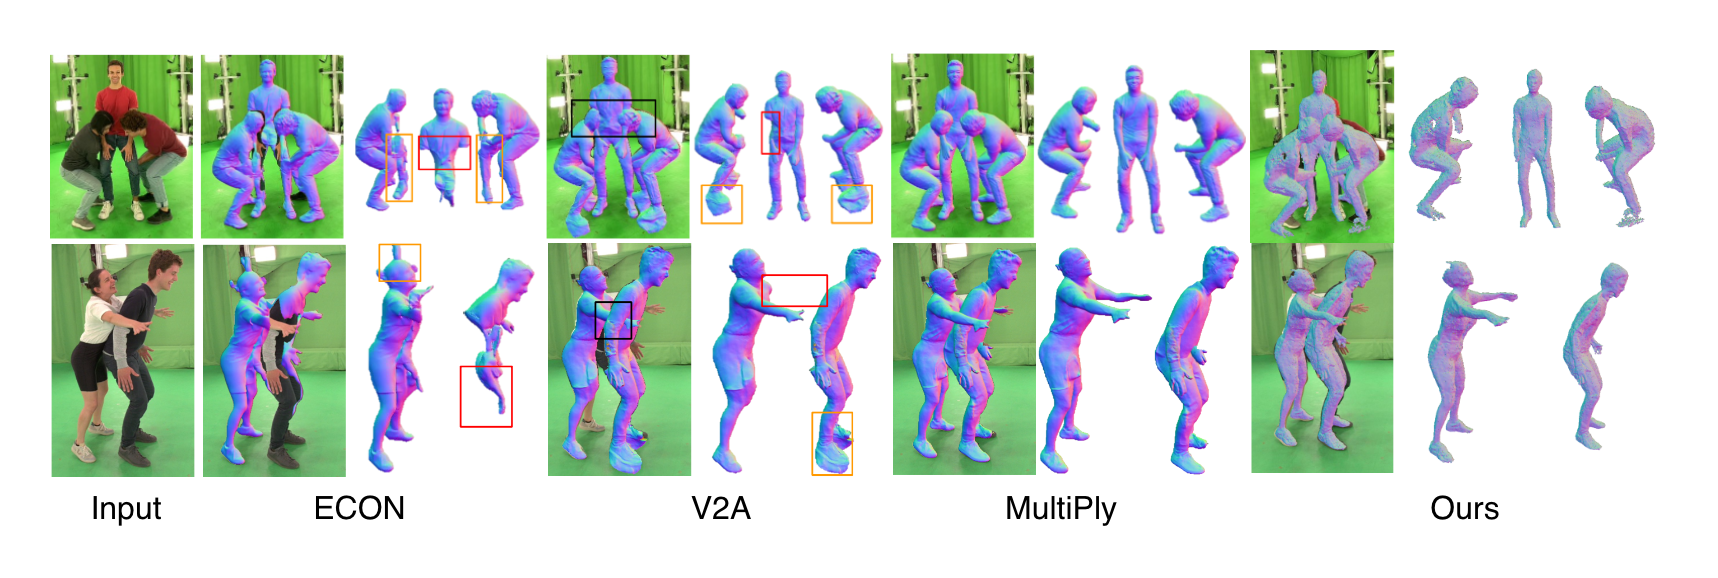
\includegraphics[width=1.0\textwidth]{figures/qual_recon_comp.drawio.png}
    \caption{\textbf{Qualitative reconstruction comparison}. We adopt the figure from MultiPly \cite{multiply} and added our reconstruction results for comparison on chosen scenes from Hi4D and MMM. For each method, we show RGB frame overlaid with a surface normal map. In addition, we also show normal maps for each person separately. The red bounding boxes show missing mesh parts due to occlusion, while the orange bounding boxes highlight extra mesh artifacts caused by poor segmentation.}
    \label{fig:qual_recon_comp}  
\end{figure}

\begin{table}[!ht]
  \centering
  \small
  \setlength{\tabcolsep}{7pt}
  \begin{tabular}{ll
      S[table-format=1.3]
      S[table-format=1.2]
      S[table-format=1.2]
      S[table-format=1.3]}
    \toprule
    \textbf{Dataset} & \textbf{Method} & \multicolumn{1}{c}{\textbf{V-IoU} $\uparrow$} & \multicolumn{1}{c}{\textbf{C-$\ell_2$} $\downarrow$} & \multicolumn{1}{c}{\textbf{P2S} $\downarrow$} & \multicolumn{1}{c}{\textbf{NC} $\uparrow$} \\
    \midrule
    Hi4D & ECON & \textit{0.787} & 3.72 & 3.59 & 0.746 \\
     & V2A & 0.783 & \textit{3.02} & 2.46 & 0.775 \\  
     & MultiPly & \textbf{0.816} & \textbf{2.53} & \textit{2.34} & \textbf{0.789} \\
     & Ours & 0.594 & 4.33 & \textbf{2.25} & \textit{0.783} \\
    \midrule
    MMM & ECON & 0.760 & 4.17 & 3.71 & 0.705 \\
     & V2A & \textit{0.812} & \textit{3.34} & \textit{2.68} & \textit{0.735} \\ 
     & MultiPly & \textbf{0.826} & \textbf{2.89} & \textbf{2.40} & \textbf{0.757} \\
     & Ours & 0.315 & 6.42 & 3.77 & 0.672 \\
    \bottomrule
  \end{tabular}
  \caption{\textbf{Human mesh reconstruction results on Hi4D and MMM.} Best results per dataset and metric are in bold, second best are in italics.}
  \label{tab:reconstruction_results}
\end{table}

We compare our mesh reconstruction quality to MultiPly \cite{multiply} and additionally report ECON \cite{econ} and Vid2Avatar (V2A) \cite{guo2023vid2avatar} as reference baselines used in MultiPly. As Table~\ref{tab:reconstruction_results} shows, MultiPly achieves the best scores on most reconstruction metrics, while our method generally trails and degrades further on MMM, which contains more people and dynamic camera motion. One exception is Hi4D P2S, where our method achieves the best score.

We attribute the remaining gap mainly to two factors. First, residual pose errors can place the posed 3DGS in a suboptimal configuration, which directly affects mesh extraction and surface metrics. Second, MultiPly reconstructs an implicit signed distance field that is designed for surface extraction, whereas our explicit 3DGS is optimized for rendering and we extract meshes via TSDF fusion of rendered depth maps, which provides an indirect and approximate geometry signal. Overall, these results suggest that the current pipeline is not yet competitive for high-fidelity geometry, and that improving pose refinement and surface extraction is the most direct direction for future work.

Figure~\ref{fig:qual_recon_comp} is consistent with the quantitative reconstruction results. Our method recovers the coarse body geometry and, in the shown examples, avoids severe missing-body artifacts under occlusion (red boxes). However, fine surface details are often smoothed out, and the extracted meshes can exhibit artifacts, which we attribute to extracting a surface via TSDF fusion from depth rendered by a rendering-optimized 3DGS representation rather than directly optimizing a watertight surface representation. In the upper row, we additionally observe spurious geometry around the right person's left foot.


\subsection{Pose Estimation Comparisons}

% selected scene and frames for this qual vis:
%  Pair15 - frame 87, Pai19 - frame 132

\begin{figure}[!ht]
    \centering
    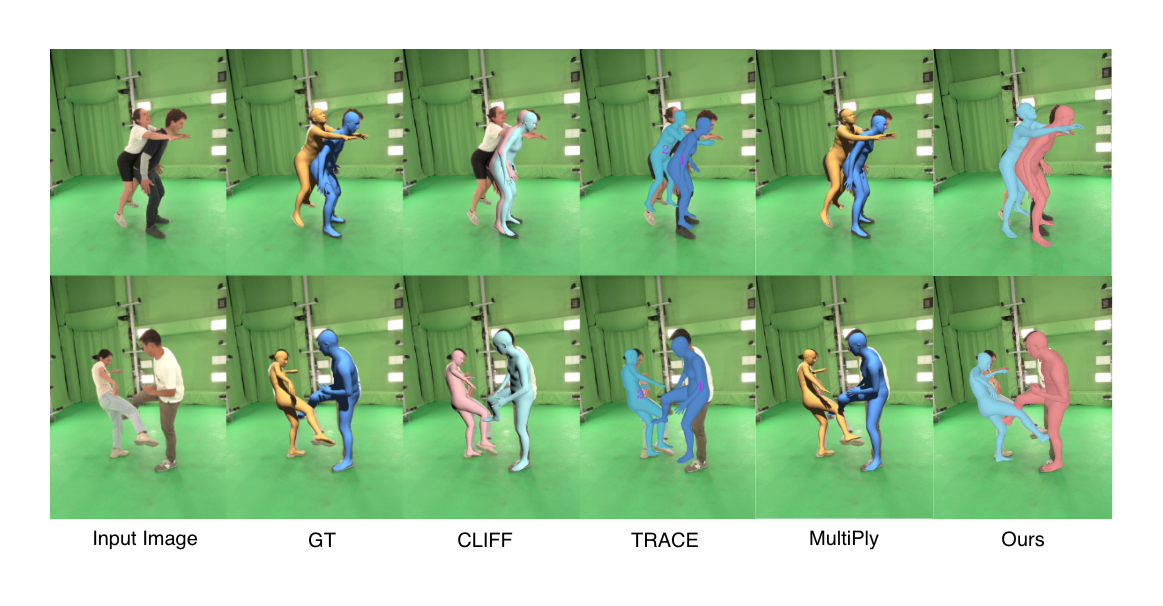
\includegraphics[width=1.0\textwidth]{figures/qual_pose_comp.drawio.png}
    \caption{\textbf{Qualitative pose estimation comparison}. We adopt the figure from MultiPly \cite{multiply} and added our pose estimation results for comparison on chosen scenes from Hi4D. For each method, we show RGB frame overlaid with predicted SMPL-(X) mesh.}
    \label{fig:qual_pose_comp}  
\end{figure}

\begin{table}[!ht]
  \centering
  \small
  \setlength{\tabcolsep}{6pt}
  \sisetup{detect-weight=true,detect-family=true}
  \begin{tabular}{c|c}
    \begin{tabular}{l
        S[table-format=2.1]
        S[table-format=3.1]
        S[table-format=3.1]
        S[table-format=1.3]}
      \toprule
      \multicolumn{5}{c}{\textbf{SMPL metrics}} \\
      \midrule
      \textbf{Method} &
      \multicolumn{1}{c}{\textbf{MPJPE} $\downarrow$} &
      \multicolumn{1}{c}{\textbf{MVE} $\downarrow$} &
      \multicolumn{1}{c}{\textbf{CD} $\downarrow$} &
      \multicolumn{1}{c}{\textbf{PCDR} $\uparrow$} \\
      \midrule
      CLIFF & 85.7 & 102.1 & 351.7 & 0.606 \\
      TRACE & 95.6 & 115.7 & 249.4 & 0.603 \\
      MultiPly & \textbf{69.4} & \textbf{83.6} & 218.4 & \textbf{0.709} \\
      H3R$^{\dagger}$ & 103.0 & 85.2 & 195.8 & 0.647 \\
      Ours$^{\dagger}$ & 102.3 & 83.8 & \textbf{189.2} & 0.634 \\
      \bottomrule
    \end{tabular}
    &
    \begin{tabular}{l
        S[table-format=2.1]
        S[table-format=2.1]
        S[table-format=1.4]}
      \toprule
      \multicolumn{4}{c}{\textbf{SMPL-X metrics}} \\
      \midrule
      \textbf{Method} &
      \multicolumn{1}{c}{\textbf{MPJPE} $\downarrow$} &
      \multicolumn{1}{c}{\textbf{MVE} $\downarrow$} &
      \multicolumn{1}{c}{\textbf{PCDR} $\uparrow$} \\
      \midrule
      CLIFF & \multicolumn{1}{c}{---} & \multicolumn{1}{c}{---} & \multicolumn{1}{c}{---} \\
      TRACE & \multicolumn{1}{c}{---} & \multicolumn{1}{c}{---} & \multicolumn{1}{c}{---} \\
      MultiPly & \multicolumn{1}{c}{---} & \multicolumn{1}{c}{---} & \multicolumn{1}{c}{---} \\
      Human3R & 80.7 & 65.9 & {\bfseries 0.617} \\
      Ours & {\bfseries 77.4} & {\bfseries 63.8} & 0.613 \\
      \bottomrule
    \end{tabular}
  \end{tabular}
	  \caption{\textbf{Human pose estimation results on Hi4D.} The left table reports SMPL-space metrics and the right table reports SMPL-X-space metrics. Best results are in bold. $^{\dagger}$ For Human3R and our method, SMPL metrics are computed after converting predicted SMPL-X parameters to SMPL (SMPL-X$\rightarrow$SMPL transfer).}
  \label{tab:pose_results_hi4d}
\end{table}

We compare our pose estimation results to MultiPly \cite{multiply} and include for reference CLIFF \cite{li2022cliff} and TRACE \cite{trace} as reported by MultiPly. We use Human3R \cite{chen2025human3r} during preprocessing to obtain the initial SMPL-X poses. Table~\ref{tab:pose_results_hi4d} reports pose metrics computed against different ground-truth parameterizations. The left table reports metrics computed against the ground-truth SMPL poses. For Human3R and our method, these are computed after converting predicted SMPL-X parameters to SMPL (SMPL-X$\rightarrow$SMPL transfer). The right table reports metrics computed against ground-truth SMPL-X poses obtained by transferring the ground-truth SMPL poses to SMPL-X, and is therefore only available for Human3R and our method which both predict SMPL-X parameters directly.

In SMPL space, MultiPly achieves the best MPJPE and PCDR, indicating more accurate joint locations and depth ordering. Our method is competitive on MVE and achieves the lowest CD, suggesting better reproduction of inter-person contact distances, but MPJPE remains the main gap compared to MultiPly. Compared to the Human3R initialization, pose tuning improves MPJPE, MVE, and CD in both SMPL and SMPL-X space, while PCDR remains slightly lower.

Figure~\ref{fig:qual_pose_comp} provides a qualitative comparison between the Human3R initialization and our pose-tuned results. In both shown scenes, pose tuning improves the alignment between the RGB frame and the rendered SMPL-X mesh compared to Human3R, supporting the effectiveness of our refinement also qualitatively.

Compared to MultiPly, the bottom-row example highlights a practical benefit of using SMPL-X rather than SMPL, as the subject's hand articulation is better captured by our SMPL-X-based predictions, whereas MultiPly's SMPL-based fit results in a more neutral hand pose. At the same time, the bottom row also shows that our method can still suffer from interpenetration between the reconstructed meshes.

\subsection{Novel View Synthesis Comparisons}

% selected scene and frames for this qual vis:
% Pair 16 - frame 66, Pair 15 - frame 90
\begin{figure}[!ht]
    \centering
    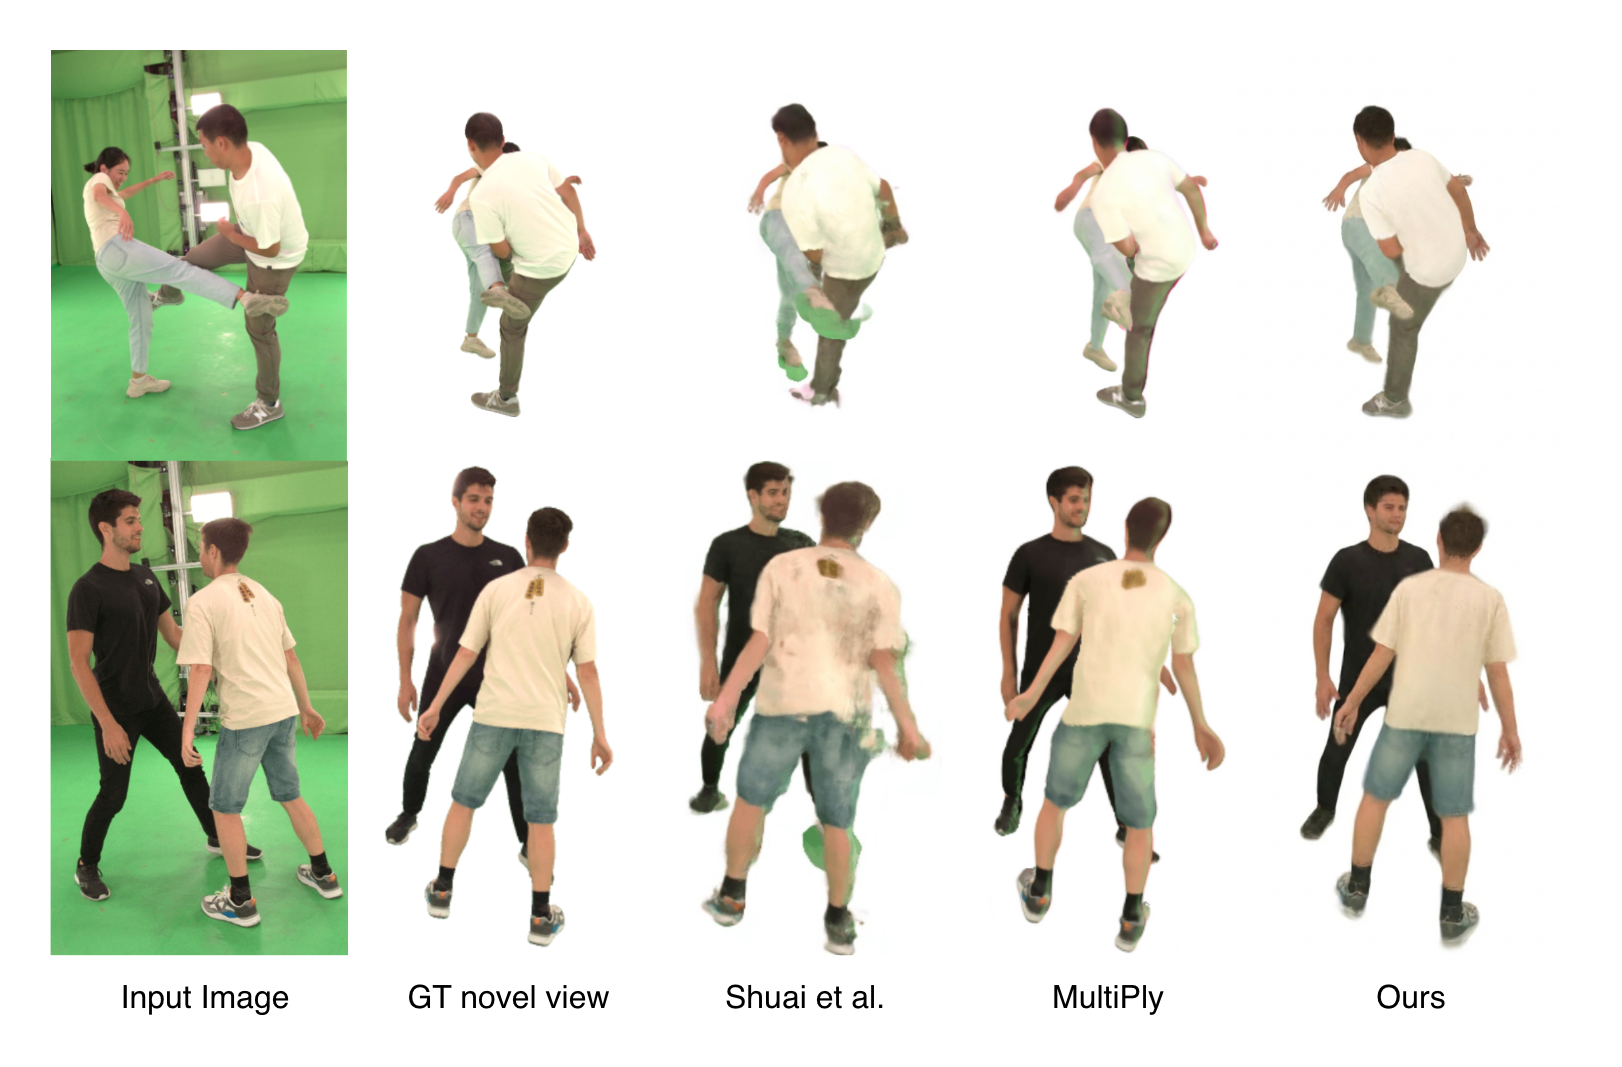
\includegraphics[width=1.0\textwidth]{figures/qual_nvs_comp.drawio.png}
    \caption{\textbf{Qualitative novel view synthesis comparison}. We adapt the figure from MultiPly \cite{multiply} and show the original source camera view along with the ground truth novel view and predictions from our method and relevant baselines.}
    \label{fig:qual_nvs_comp}  
\end{figure}

\begin{table}[!ht]
  \centering
  \small
  \setlength{\tabcolsep}{7pt}
  \begin{tabular}{l
      S[table-format=1.3]
      S[table-format=2.1]
      S[table-format=1.4]}
    \toprule
    \textbf{Method} & \multicolumn{1}{c}{\textbf{SSIM} $\uparrow$} & \multicolumn{1}{c}{\textbf{PSNR} $\uparrow$} & \multicolumn{1}{c}{\textbf{LPIPS} $\downarrow$} \\
    \midrule
    Shuai et al. & 0.898 & 19.6 & 0.1099 \\
    MultiPly & 0.915 & \textbf{20.7} & \textbf{0.0798} \\
    Ours & \textbf{0.926} & 20.1 & 0.0809 \\
    \bottomrule
  \end{tabular}
  \caption{\textbf{Novel view synthesis results on Hi4D.} Best results are in bold.}
  \label{tab:nvs_results_hi4d}
\end{table}


In addition to MultiPly, we also compare to Shuai et al. \cite{nv_interact}, a multi-view method that was adapted by MultiPly to work in a monocular setting. Under the masked, downscaled evaluation protocol described above, our method achieves the best SSIM, while MultiPly achieves the best PSNR and LPIPS. Overall, these results suggest that our novel view synthesis quality is broadly on par with MultiPly. Structural similarity is slightly better for our method, LPIPS is only slightly worse, and the main difference is PSNR, which emphasizes pixel-wise differences. Taken together, the gap largely boils down to pixel-level discrepancies rather than a clear difference in perceptual or structural quality.

Figure \ref{fig:qual_nvs_comp} provides qualitative novel view synthesis comparisons. In the bottom-row example, our method preserves the head shape of the subject closer to the camera and produces sharper local details than MultiPly. This sharpening may partially explain why our PSNR is slightly lower, as PSNR is sensitive to pixel-wise differences even when images appear perceptually crisp. At the same time, MultiPly better preserves the tag on the back of the subject, which we attribute to our initialization. Since LHM observes the person from essentially a single view, details that are never visible (such as a back-facing tag) may not be reconstructed reliably and therefore cannot be reinforced through backpropagation during training. Finally, in the top-row example, MultiPly exhibits greenish color artifacts that are likely caused by background pixels leaking into the foreground during progressive mask refinement. We do not observe these artifacts in our renderings, which we attribute to refining synthesized training views with DiFix, helping to suppress such mask-related color leakage.

\subsection{Training Speed}

\begin{table}[!ht]
  \centering
  \small
  \setlength{\tabcolsep}{7pt}
  \sisetup{detect-weight=true,detect-family=true}
  \begin{tabular}{c
      S[table-format=2.1]
      S[table-format=2.1]
      S[table-format=2.1]}
    \toprule
    \textbf{Input Frames} & \multicolumn{1}{c}{\textbf{DiFix [min]}} & \multicolumn{1}{c}{\textbf{Optimization [min]}} & \multicolumn{1}{c}{\textbf{Total [min]}} \\
    \midrule
    50  & 5.8  & 8.5  & 14.3 \\
    100 & 11.7 & 16.9 & 28.6 \\
    200 & 23.3 & 33.8 & 57.1 \\
    \bottomrule
  \end{tabular}
  \caption{\textbf{Training speed breakdown} on a single NVIDIA V100 at $\approx 980\times1280$ resolution and batch size 5. \textbf{DiFix} is the time to synthesize $7$ novel cameras for $F/5$ timestamps at $5\,\text{s}$ per frame. \textbf{Optimization} is an estimate based on $1.3\,\text{s}$ per update and our two-stage schedule (15 epochs on $F$ source frames, then 15 epochs on $8\cdot(F/5)$ training images). Timings exclude preprocessing (Human3R/SAM3/LHM).}
  \label{tab:training_speed_breakdown}
\end{table}

An advantage of our 3DGS-based pipeline is training efficiency. On a single NVIDIA V100 and input resolution $\approx 980 \times 1280$ with batch size 5, a single optimization step takes $1.3\,\text{s}$. In addition, our pipeline synthesizes novel training views using DiFix. Synthesizing one novel frame takes $5\,\text{s}$. We synthesize $7$ novel cameras and use a temporally downsampled set of training timestamps (downsample factor $5$). For a monocular video with $F$ frames, this corresponds to approximately $F/5$ training timestamps per camera, i.e.

\begin{equation}
T_{\text{DiFix}} \approx 5\,\text{s} \cdot 7 \cdot \frac{F}{5}.
\end{equation}

\noindent Table~\ref{tab:training_speed_breakdown} summarizes the resulting overhead from DiFix and provides an approximate end-to-end runtime. We estimate optimization time under our two-stage training schedule. During the first 15 epochs (pose tuning), we optimize on the full monocular video (one source view, $F$ frames). During the remaining 15 epochs (3DGS optimization), we optimize on the subsampled training set with one source view and seven synthesized views at $F/5$ timestamps, i.e. $8\cdot(F/5)$ training images per epoch. We assume batch size 5 and $1.3\,\text{s}$ per optimization step.



\noindent In contrast, MultiPly reports a runtime on the order of one day per person \cite{multiply}. While this comparison is not directly controlled for hardware and implementation details, it highlights that our approach can provide competitive quality at substantially lower training cost.


\subsection{Ablation Study: Novel Training View Synthesis Components}

To isolate the impact of the novel training view synthesis components and avoid confounding effects from pose refinement, we disable pose tuning for all experiments in this ablation.

\begin{table}[!ht]
  \centering
  \small
  \setlength{\tabcolsep}{7pt}
  \begin{tabular}{c
      c
      l
      S[table-format=1.3]
      S[table-format=2.1]
      S[table-format=1.4]}
    \toprule
    \textbf{LHM Init} & \textbf{DiFix} & \textbf{Reference Camera} & \multicolumn{1}{c}{\textbf{SSIM} $\uparrow$} & \multicolumn{1}{c}{\textbf{PSNR} $\uparrow$} & \multicolumn{1}{c}{\textbf{LPIPS} $\downarrow$} \\
    \midrule
    $\checkmark$ & $\times$ & - & 0.925 & 20.0 & \textbf{0.0818} \\
    \midrule
    $\times$ & $\times$ & - & 0.890 & 17.0 & 0.1343 \\
    $\times$ & $\checkmark$ & Source & 0.903 & 17.1 & 0.1184 \\
    $\times$ & $\checkmark$ & Previous & 0.900 & 17.0 & 0.1206 \\
    $\checkmark$ & $\checkmark$ & Source & \textbf{0.926} & \textbf{20.2} & 0.0865 \\
    $\checkmark$ & $\checkmark$ & Previous & \textbf{0.926} & \textbf{20.2} & 0.0872 \\
    \bottomrule
  \end{tabular}
  \caption{\textbf{Ablation study on novel view synthesis.} Results are reported under the same evaluation protocol as Table~\ref{tab:nvs_results_hi4d}. The \textbf{LHM Init} and \textbf{DiFix} columns indicate whether the corresponding component is enabled. Best results are in bold.}
  \label{tab:ablation_nvs}
\end{table}

\noindent Table~\ref{tab:ablation_nvs} isolates the impact of (i) LHM initialization, (ii) DiFix-based refinement of synthesized novel training views, and (iii) the choice of reference camera for DiFix (source view versus the previously synthesized view). Training without LHM initialization and without any view synthesis performs worst, highlighting that learning a renderable representation from strictly monocular supervision is challenging under our compute budget. Adding novel training views that are rendered from the partially trained model and refined with DiFix yields only a modest improvement in this setting.

\noindent LHM initialization is the dominant factor: simply initializing from LHM (without DiFix) substantially improves all metrics and provides the best LPIPS in our ablation. Adding DiFix refinement on top of LHM leads to only marginal changes: SSIM and PSNR improve slightly, while LPIPS becomes worse. Figure~\ref{fig:qual_difix_comp} provides an explanation for this behavior. Without LHM initialization, the intermediate renders are substantially degraded, which gives DiFix too much freedom during refinement. In both reference strategies, this leads to implausible hallucinations, such as an incorrect rotation of the head. With LHM initialization, the renders are already significantly closer to the target view, and DiFix mainly acts as a detail enhancement module, sharpening local texture without correcting higher-level geometric errors. Finally, using the source camera versus the previous synthesized camera as the DiFix reference yields very similar results, with a slight advantage for the source-reference strategy, suggesting that potential error accumulation in the chained (previous-reference) strategy can offset the benefit of higher overlap. Despite the small advantage of the source-reference strategy in this ablation, we use the previous-reference strategy in our main pipeline, as we expect it to benefit more from the higher inter-view overlap when the refinement model is stronger and produces less drift.

\begin{figure}[!ht]
    \centering
    \includegraphics[width=0.9\textwidth]{figures/qual_difix_comp.drawio.png}
    \caption{\textbf{Qualitative comparison of novel training view synthesis}. We show comparison of novel view synthesis strategies along the following axis: (i) LHM initialization vs. random initialization, and (ii) DiFix refinement using source view vs. previous view. In total, we show four possible configurations. In each configuration, we show the reference view (left column), the rendered view to be refined (middle column), and the refined view by DiFix (right column).}
    \label{fig:qual_difix_comp}  
\end{figure}

\begin{figure}[!ht]
    \centering
    \includegraphics[width=0.8\textwidth]{figures/n_trn_cameras_ablation_setup.drawio.png}
    \caption{\textbf{Distribution of the cameras for the ablation}. We show the distribution of the cameras used in the ablation study on the number of novel training cameras. The blue camera is the source camera, and the orange cameras are the novel training cameras. Specifically, we experiment with 0, 2, 4, and 7 novel training cameras.}
    \label{fig:n_trn_cameras_ablation_setup}  
\end{figure}


% We will skip this for now since it adds little value compared to the table and the other fig
% \begin{figure}[!ht]
    % \centering
    % \includegraphics[width=1.0\textwidth]{figures/qual_diff_trn_nv_strategies.drawio.png}
    % \caption{\textbf{Qualitative comparison of synthesised novel views based on different novel view training strategies}. First row: no training novel cameras synthesised, novel training cameras synthesised using either source or previous camera as reference. Second row: synthesised view of the LHM initialized 3DGS, novel training cameras synthesised using either source or previous camera as reference.}
    % \label{fig:qual_comp_trn_nvs_strategies}  
% \end{figure}

\subsection{Ablation Study: Number of Novel Training Cameras}

\begin{table}[!ht]
  \centering
  \small
  \setlength{\tabcolsep}{7pt}
  \begin{tabular}{c
      S[table-format=1.3]
      S[table-format=2.1]
      S[table-format=1.4]}
    \toprule
    \textbf{Number of Novel Training Cameras} & \multicolumn{1}{c}{\textbf{SSIM} $\uparrow$} & \multicolumn{1}{c}{\textbf{PSNR} $\uparrow$} & \multicolumn{1}{c}{\textbf{LPIPS} $\downarrow$} \\
    \midrule
    0 & 0.908 & 18.8 & 0.1134 \\
    2 & 0.922 & 20.1 & 0.0953 \\
    4 & 0.925 & \textbf{20.3} & 0.0903 \\
    7 & \textbf{0.926} & 20.2 & \textbf{0.0872} \\
    \bottomrule
  \end{tabular}
  \caption{\textbf{Ablation study on number of novel training cameras}. Best results are in bold.}
  \label{tab:ablation_num_trn_cams}
\end{table}

One motivation for introducing DiFix-based novel training view synthesis is that optimizing a 3DGS model from monocular video requires multi-view supervision. Without additional views, we expect poor novel view synthesis performance, even when starting from an LHM initialization, because subsequent monocular fine-tuning can overfit to the single source view. To test this assumption, we ablate the number of novel training cameras used during training. We consider 0, 2, 4, and 7 novel training cameras, where 0 means training uses only the source camera. All experiments are initialized from LHM when novel cameras are used, their training images are synthesized and refined with DiFix.
Similar to the previous section, we again disable pose tuning for all experiments. Finally, Figure~\ref{fig:n_trn_cameras_ablation_setup} shows the camera distribution used in this ablation.

Table~\ref{tab:ablation_num_trn_cams} confirms our hypothesis. Using 0 novel training cameras performs substantially worse across all metrics, indicating that monocular fine-tuning alone is insufficient despite the strong LHM initialization. Adding just 2 novel training cameras yields a large improvement, while increasing from 2 to 4 and 7 yields diminishing returns. Overall, 7 cameras achieves the best SSIM and LPIPS, while PSNR peaks at 4 cameras with a small difference to 7. Despite these diminishing returns, we decided to use 7 novel training cameras in our main pipeline to maximize multi-view supervision during training.

\subsection{Ablation Study: Pose Optimization During 3DGS Training}

\begin{table}[!ht]
  \centering
  \small
  \setlength{\tabcolsep}{6pt}
  \sisetup{detect-weight=true,detect-family=true}
  \begin{tabular}{l
      S[table-format=2.4]
      S[table-format=2.4]
      S[table-format=1.4]
      |
      S[table-format=1.3]
      S[table-format=2.1]
      S[table-format=1.4]}
    \toprule
    \textbf{Section} &
    \multicolumn{1}{c}{\textbf{MPJPE [mm]} $\downarrow$} &
    \multicolumn{1}{c}{\textbf{MVE [mm]} $\downarrow$} &
    \multicolumn{1}{c}{\textbf{PCDR} $\uparrow$} &
    \multicolumn{1}{c}{\textbf{SSIM} $\uparrow$} &
    \multicolumn{1}{c}{\textbf{PSNR} $\uparrow$} &
    \multicolumn{1}{c}{\textbf{LPIPS} $\downarrow$} \\
    \midrule
    No Pose Tuning & 80.7000 & 65.9000 & {\bfseries 0.6170} & {\bfseries 0.926} & {\bfseries 20.2} & 0.0872 \\
    \midrule
    A (baseline) & {\bfseries 77.4410} & 63.7939 & 0.6133 & {\bfseries 0.926} & 20.1 & 0.0809 \\
    B (interpenetration) & 77.5931 & 63.4099 & 0.6123 & {\bfseries 0.926} & 20.1 & 0.0809 \\
    C (depth-order) & 77.9943 & 63.6916 & 0.6099 & 0.925 & 20.0 & 0.0818 \\
    D (confidence-guided) & 77.6290 & 63.4303 & 0.6123 & {\bfseries 0.926} & 20.1 & {\bfseries 0.0808} \\
    E (hands) & 77.5986 & {\bfseries 63.4009} & 0.6123 & {\bfseries 0.926} & 20.1 & 0.0809 \\
    \bottomrule
  \end{tabular}
  \caption{\textbf{Pose optimization ablation study (Hi4D average across scenes)}. We report SMPL-X pose metrics (MPJPE/MVE/PCDR) and novel view synthesis (SSIM/PSNR/LPIPS). For each section (A-E), we list the best-performing experiment.} % todo: add reference here to the section in appendix where we add the full hyper parameter study
  \label{tab:ablation_pose_opt}
\end{table}

\paragraph{Ablation setting.} Accurate pose estimation is crucial for realistic reconstruction of interacting humans, yet it remains challenging in close interactions. We therefore explore pose tuning during 3DGS training and evaluate its effect on both pose accuracy and novel view synthesis (NVS). Section A in Table~\ref{tab:ablation_pose_opt} tunes \texttt{root\_pose}, \texttt{body\_pose}, \texttt{trans} and \texttt{betas} which is also what we use in our main experiments. We further explore three additional loss/optimization components from prior work ( Sections B-D) and the effect of adding hand parameters to the optimized SMPL-X parameter set (Section E). For each section, we perform a small hyperparameter sweep and report the best-performing configuration.

\paragraph{Interpenetration Loss.} First, we adopt the interpenetration loss introduced in Remips \cite{remips}, where it is applied to naked human body models. In contrast, we adapt this term to our 3DGS human representation as follows. Given a set of Gaussians for each person, we subsample their centers to make the computation feasible (by default, we use 2000 points per person). For two people A and B, and their subsampled Gaussian centers $\{pA_i\}_{i=1}^{N_A}$ and $\{pB_j\}_{j=1}^{N_B}$, we define the displacement vector between a pair of centers as $d_{ij} = pA_i - pB_j$ and the corresponding distance as $\lVert d_{ij} \rVert_2$. We compare this distance to an allowed margin $m_{ij} = rA_i + rB_j + \delta$, where $rA_i$ and $rB_j$ are the radii of the two Gaussians and $\delta$ is a small constant margin (by default set to 0.03\,m). The interpenetration loss is defined as

\begin{equation}
\mathcal{L}_{\text{inter}}(A,B) =
\frac{1}{N_A N_B}
\sum_{i=1}^{N_A}\sum_{j=1}^{N_B}
\max\left(0, m_{ij} - \lVert d_{ij} \rVert_2\right),
\end{equation}

\noindent where $N_A$ and $N_B$ denote the number of subsampled Gaussian centers for person A and B.

\paragraph{Depth Order Loss.} Second, we adopt the depth order loss from MultiPly \cite{multiply}. We use individual person masks from SAM3 as a per-pixel assignment signal and compare this assignment to the rendered depths of each person. If the person selected by the mask is not the front-most person according to the rendered depths, we apply a penalty. In practice, we exclude pixels with ambiguous assignments (e.g., overlapping masks) and compute the loss only on pixels that can be confidently attributed to a single person.

More precisely, for every pixel $(u,v)$ with reliable mask information, we first obtain the rendered depth of the person selected by the SAM3 masks, denoted as $d_{\text{mask}}(u,v)$. We then obtain the minimum rendered depth across all people at that pixel, denoted as $d_{\text{min}}(u,v)$. Finally, we compute the depth order loss for a given pixel as

\begin{equation}
\mathcal{L}_{\text{depth}}(u,v) = \operatorname{softplus}\left(d_{\text{mask}}(u,v) - d_{\text{min}}(u,v)\right),
\end{equation}


\noindent where $\operatorname{softplus}(x) = \log(1+\exp(x))$. Finally, we average this loss over all pixels where we have mask information.

\paragraph{Confidence Guided Optimization.} In general, it is not desirable to optimize our 3DGS model on frames where the pose estimation is poor, as this would encourage the model to explain the input with incorrect poses. Similarly, we would like to avoid adjusting shape parameters when pose estimates are unreliable. Therefore, we adapt MultiPly's confidence-guided optimization strategy \cite{multiply} and split frames into reliable and unreliable according to the following criterion. We render each person in each frame and use the accumulated opacity to define the person's 2D silhouette. We then compute the IoU between this silhouette and the corresponding SAM3 mask. We repeat this for every person in the frame and average the IoUs to obtain a frame-level confidence score. If this score is above a threshold (by default set to 0.75), we consider the frame reliable. We update this reliability status every 5 epochs. During the pose optimization phase, we optimize pose and shape parameters on reliable frames, while we optimize only pose on unreliable frames. After pose optimization is finished, we use only reliable frames to generate novel training views for the subsequent 3DGS optimization phase, and discard unreliable frames for 3DGS training.

\begin{figure}[!ht]
    \centering
    \includegraphics[width=1.0\textwidth]{figures/qual_tune_and_notune_pose.drawio.png}
    \caption{\textbf{Qualitative comparison of using pose tuning}. The first two columns show the rendered 3DGS overlaid on the GT image. We highlight (red box) a strong misalignment caused by inaccurate pose. The last two columns show only the GT mesh (blue) and the estimated mesh (orange).}
    \label{fig:qual_tune_and_notune_pose}  
\end{figure}


\paragraph{Interpretation of Pose Results.} Table~\ref{tab:ablation_pose_opt} summarizes the results of our pose optimization ablation study. Pose tuning improves MPJPE and MVE compared to no pose tuning, confirming that optimizing pose during 3DGS training can improve pose accuracy. At the same time, the best PCDR is achieved by the \textit{No Pose Tuning} setting. This suggests that our pose tuning improves joint/vertex accuracy on average, but does not necessarily improve (and can slightly hurt) PCDR, which may be sensitive to segmentation noise and small depth inconsistencies.

Across Sections B to E, we do not observe a consistent improvement over the baseline pose-tuning configuration (Section A). The only notable change is that optimizing additional SMPL-X parameters (hands) yields the best MVE. For the interpenetration and depth-order losses, one possible explanation is that despite exploring different weights, these terms may still be underweighted relative to the other objectives, limiting their impact. For the interpenetration loss, another potential bottleneck is Gaussian subsampling, which may miss rare but important interpenetration cases. For the depth-order loss, a potential limitation is noise in the SAM3 masks, which can lead to incorrect per-pixel supervision.


\paragraph{Interpretation of the Novel View Synthesis Results.} Overall, pose optimization does not lead to a consistent improvement in novel view synthesis quality compared to no pose tuning. The largest gain is in LPIPS, suggesting that improved alignment during training can translate into perceptually better renderings (e.g., sharper appearance). Following MultiPly's evaluation protocol, we use the ground truth pose to synthesize novel views for evaluation. Therefore, improved pose estimates can only benefit NVS indirectly through better supervision during training, not through the evaluation-time rendering itself. This is illustrated in Figure~\ref{fig:qual_tune_and_notune_pose}, where pose tuning improves the alignment between the rendered 3DGS and the GT image. Better alignment during training can help the model learn more accurate color and density values, which can improve NVS even when evaluated with GT poses.


\subsection{Ablation Study: 3DGS to Mesh Conversion}

Converting the optimized 3DGS representation to a mesh is a crucial step for geometry evaluation, yet it is not trivial. We use the training pipeline outlined in the Method section for the mesh extraction experiments. In this ablation study, we explore two strategies for converting the 3DGS to a mesh. We use Marching Cubes (MC) \cite{marching_cubes} and Truncated Signed Distance Function (TSDF) fusion of rendered depth maps as implemented in Open3D \cite{open3d}.


\paragraph{3D Voxel Grid Definition from 3DGS.} In order to use MC, we first need to convert the 3DGS to a 3D voxel grid with occupancy values for each point in the 3D grid. To define the occupancy value for each of these points, we first compute the contribution of each Gaussian to the point as follows.

\begin{equation}
c_i(\mathbf{x}) =
\begin{cases}
w_i \exp\left(-\dfrac{\lVert \mathbf{x} - \boldsymbol{\mu}_i \rVert_2^2}{2\sigma_i^2}\right), & \text{if } \lVert \mathbf{x} - \boldsymbol{\mu}_i \rVert_2 \le \tau \sigma_i, \\
0, & \text{otherwise},
\end{cases}
\end{equation}

\noindent where $\mathbf{x}$ is a voxel-grid point, $\boldsymbol{\mu}_i$ is the Gaussian center, $w_i \in [0,1]$ is its opacity weight, $\sigma_i$ is its (isotropic) scale, and $\tau$ is a truncation factor (default $\tau=2.5$). The resulting occupancy (density) field is then computed by summing contributions of all Gaussians.

\begin{equation}
\rho(\mathbf{x}) = \sum_i c_i(\mathbf{x}).
\end{equation}

\noindent We repeat this for all voxel-grid points to obtain the full occupancy grid, and then apply MC with a fixed iso-surface value (default $0.07$) to extract the mesh.

\paragraph{TSDF Fusion from Rendered Depth Maps.} For TSDF fusion, we render a depth map of each person from multiple views, fuse these depth observations into a volumetric TSDF using Open3D, and extract the mesh as the zero-level set. In our implementation, we optionally apply alpha-thresholding to ignore unreliable depth values and postprocess the extracted mesh (hole filling and smoothing).

\begin{table}[!ht]
  \centering
  \small
  \setlength{\tabcolsep}{7pt}
  \sisetup{detect-weight=true,detect-family=true}
  \begin{tabular}{ll
      S[table-format=1.4]
      S[table-format=1.4]
      S[table-format=1.4]
      S[table-format=1.4]}
    \toprule
    \textbf{Dataset} & \textbf{Method} &
    \multicolumn{1}{c}{\textbf{V-IoU} $\uparrow$} &
    \multicolumn{1}{c}{\textbf{C-$\ell_2$} $\downarrow$} &
    \multicolumn{1}{c}{\textbf{P2S} $\downarrow$} &
    \multicolumn{1}{c}{\textbf{NC} $\uparrow$} \\
    \midrule
    Hi4D & TSDF & 0.5938 & {\bfseries 4.3276} & {\bfseries 2.2454} & {\bfseries 0.7831} \\
     & MC & {\bfseries 0.6329} & 4.7074 & 2.9464 & 0.6886 \\
    \midrule
    MMM & TSDF & 0.3151 & {\bfseries 6.4201} & {\bfseries 3.7659} & {\bfseries 0.6717} \\
     & MC & {\bfseries 0.4268} & 6.5439 & 3.9907 & 0.6163 \\
    \bottomrule
  \end{tabular}
  \caption{\textbf{Ablation study on 3DGS$\rightarrow$mesh conversion}. We compare TSDF fusion and Marching Cubes (MC) and report reconstruction metrics averaged across scenes. Best results per dataset and metric are highlighted in bold.}
  \label{tab:ablation_3dgs_to_mesh}
\end{table}


\begin{figure}[!ht]
    \centering
    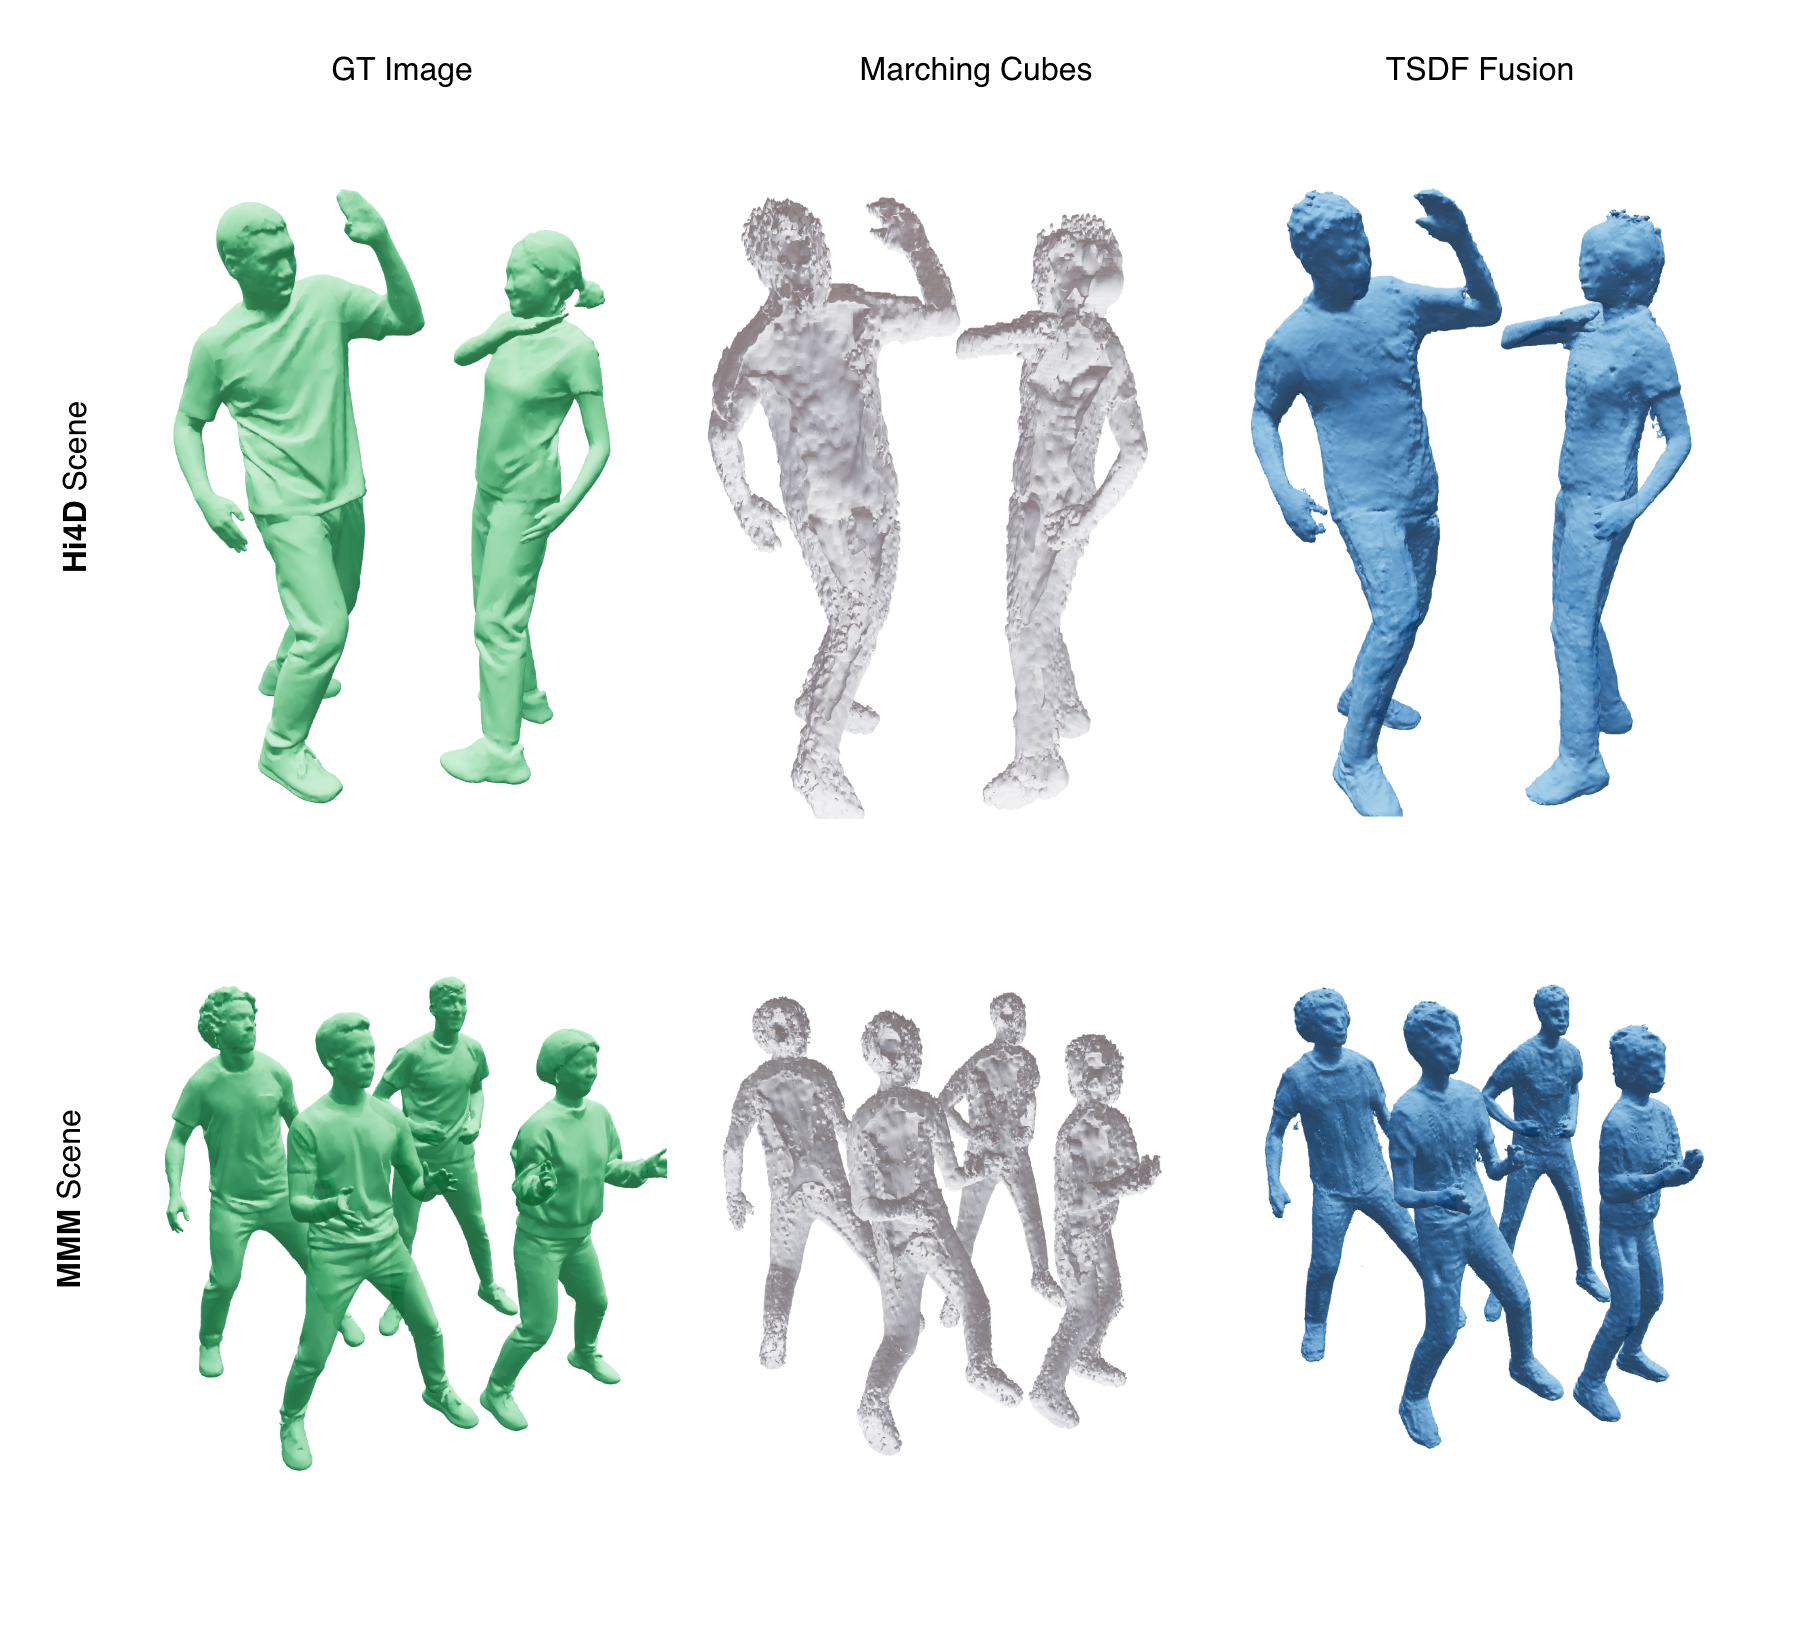
\includegraphics[width=0.75\textwidth]{figures/qual_3dgs_to_mesh.drawio.png}
    \caption{\textbf{Qualitative comparison between MC and TSDF fusion based mesh extraction}. We show the extracted meshes for each method along with the ground truth mesh for reference. First row shows selected example from the Hi4D dataset, second row shows selected example from the MMM dataset. 
    }
    \label{fig:qual_abl_3dgs_to_mesh}  
\end{figure}

\paragraph{Interpretation of the results.} Table~\ref{tab:ablation_3dgs_to_mesh} shows a clear trend across both datasets. TSDF fusion achieves better results across all metrics except for Volumetric IoU (V-IoU), where MC performs better. Figure~\ref{fig:qual_abl_3dgs_to_mesh} further supports these results qualitatively. TSDF fusion produces smoother, less blobby meshes compared to MC, and MC exhibits more holes.

Finally, results consistently degrade when moving from Hi4D to MMM. Since we render per-person depth maps for meshing, inter-person occlusions do not affect TSDF fusion directly. We hypothesize that the drop is instead driven by factors such as reduced pose accuracy (which affects the posed 3DGS) and the overall increased difficulty of MMM (more complex interactions and motion), which can lead to noisier per-person depth and occupancy estimates. Overall, these results indicate that TSDF fusion is a better choice for converting 3DGS to mesh in our pipeline, which is why we use TSDF fusion for the reconstruction results in Table~\ref{tab:reconstruction_results}.
